\chapter{Método propuesto}
\label{c:parte4}
\vspace{1cm}
En este capítulo se presenta el diseño del método propuesto sustentándose en el marco teórico introducido en el capítulo anterior. Se describen cada una de las etapas involucradas en el método, planteándose algunas técnicas para el realce de detalles y mejora de la iluminación de la imagen. Además, se presentan estrategias utilizadas para mejorar el desempeño en el tiempo de procesamiento, como así también para obtener una correcta detección del objeto en la escena.
\section{Diseño del método}
El método para el reconocimiento y seguimiento de un objeto en una secuencia de video que se propone en este trabajo consta de dos fases, cada una de ellas compuesta por varios procesos internos. Las fases pueden observarse en los diagramas de las Figs. \ref{fig:diagrama_metodo_entrenamiento} y \ref{fig:diagrama_metodo}  y las hemos definido como:
\begin{itemize}
 \item \textbf{Configuración}: la configuración se realiza una sola vez al inicio del algoritmo y es en la que se registra la imagen que posteriormente se detectará en el flujo de video. Esta etapa se encuentra representada en la Fig. \ref{fig:diagrama_metodo_entrenamiento}, la cual consta de varios procesos: primeramente, una conversión a escala de grises con una fórmula perceptualmente ponderada, luego se realiza un pre-procesamiento de iluminación y realce de detalles y finalmente, se procede con la extracción y descripción de características sobre la imagen.
 \item \textbf{Ejecución}: esta etapa contempla la captura de un frame del flujo de video proporcionado por la cámara web, el procesamiento para detectar el objeto registrado en la etapa anterior y la posterior superposición de un objeto virtual para enriquecer la realidad. Todo esto está representado en la Fig. \ref{fig:diagrama_metodo}, la cual está compuesta por diferentes procesos, entre los cuales se encuentran: la detección de movimiento, la extracción y descripción de características, la búsqueda de correspondencias (que usa como entrada la salida del proceso de configuración), la detección de la homografía y las validaciones posteriores para finalmente, en caso que la imagen patrón haya sido detectada, obtener un frame con el objeto virtual superpuesto. Estos procesos y otros que por cuestiones de brevedad no se mencionan aquí, serán descriptos en las secciones que componen este capítulo.
\end{itemize}
\begin{figure}[tbhp]
   \centering
        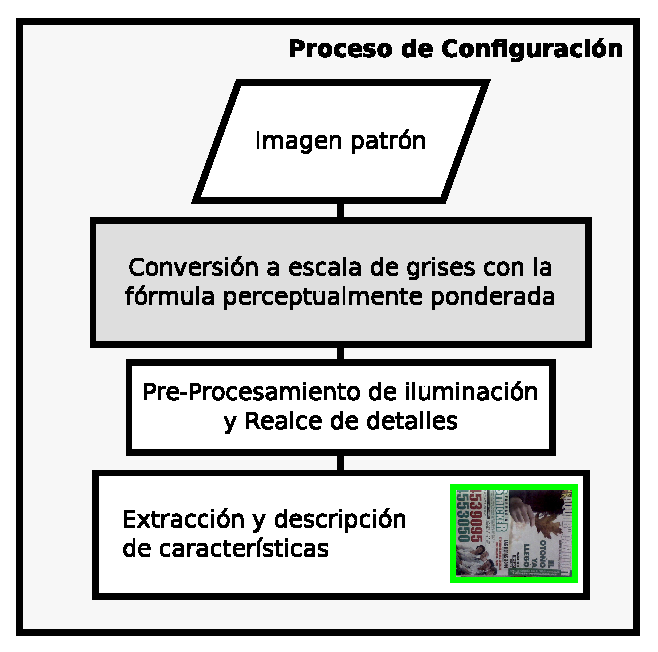
\includegraphics[scale=0.7]{../figs/proceso_completo_entrenamiento}
    \caption[Diagrama de flujo de la etapa de configuración]{Diagrama de flujo de la etapa de Configuración.}
   \label{fig:diagrama_metodo_entrenamiento}                %% Etiqueta para la figura entera
\end{figure}
\begin{figure}[tbhp]
   \centering
        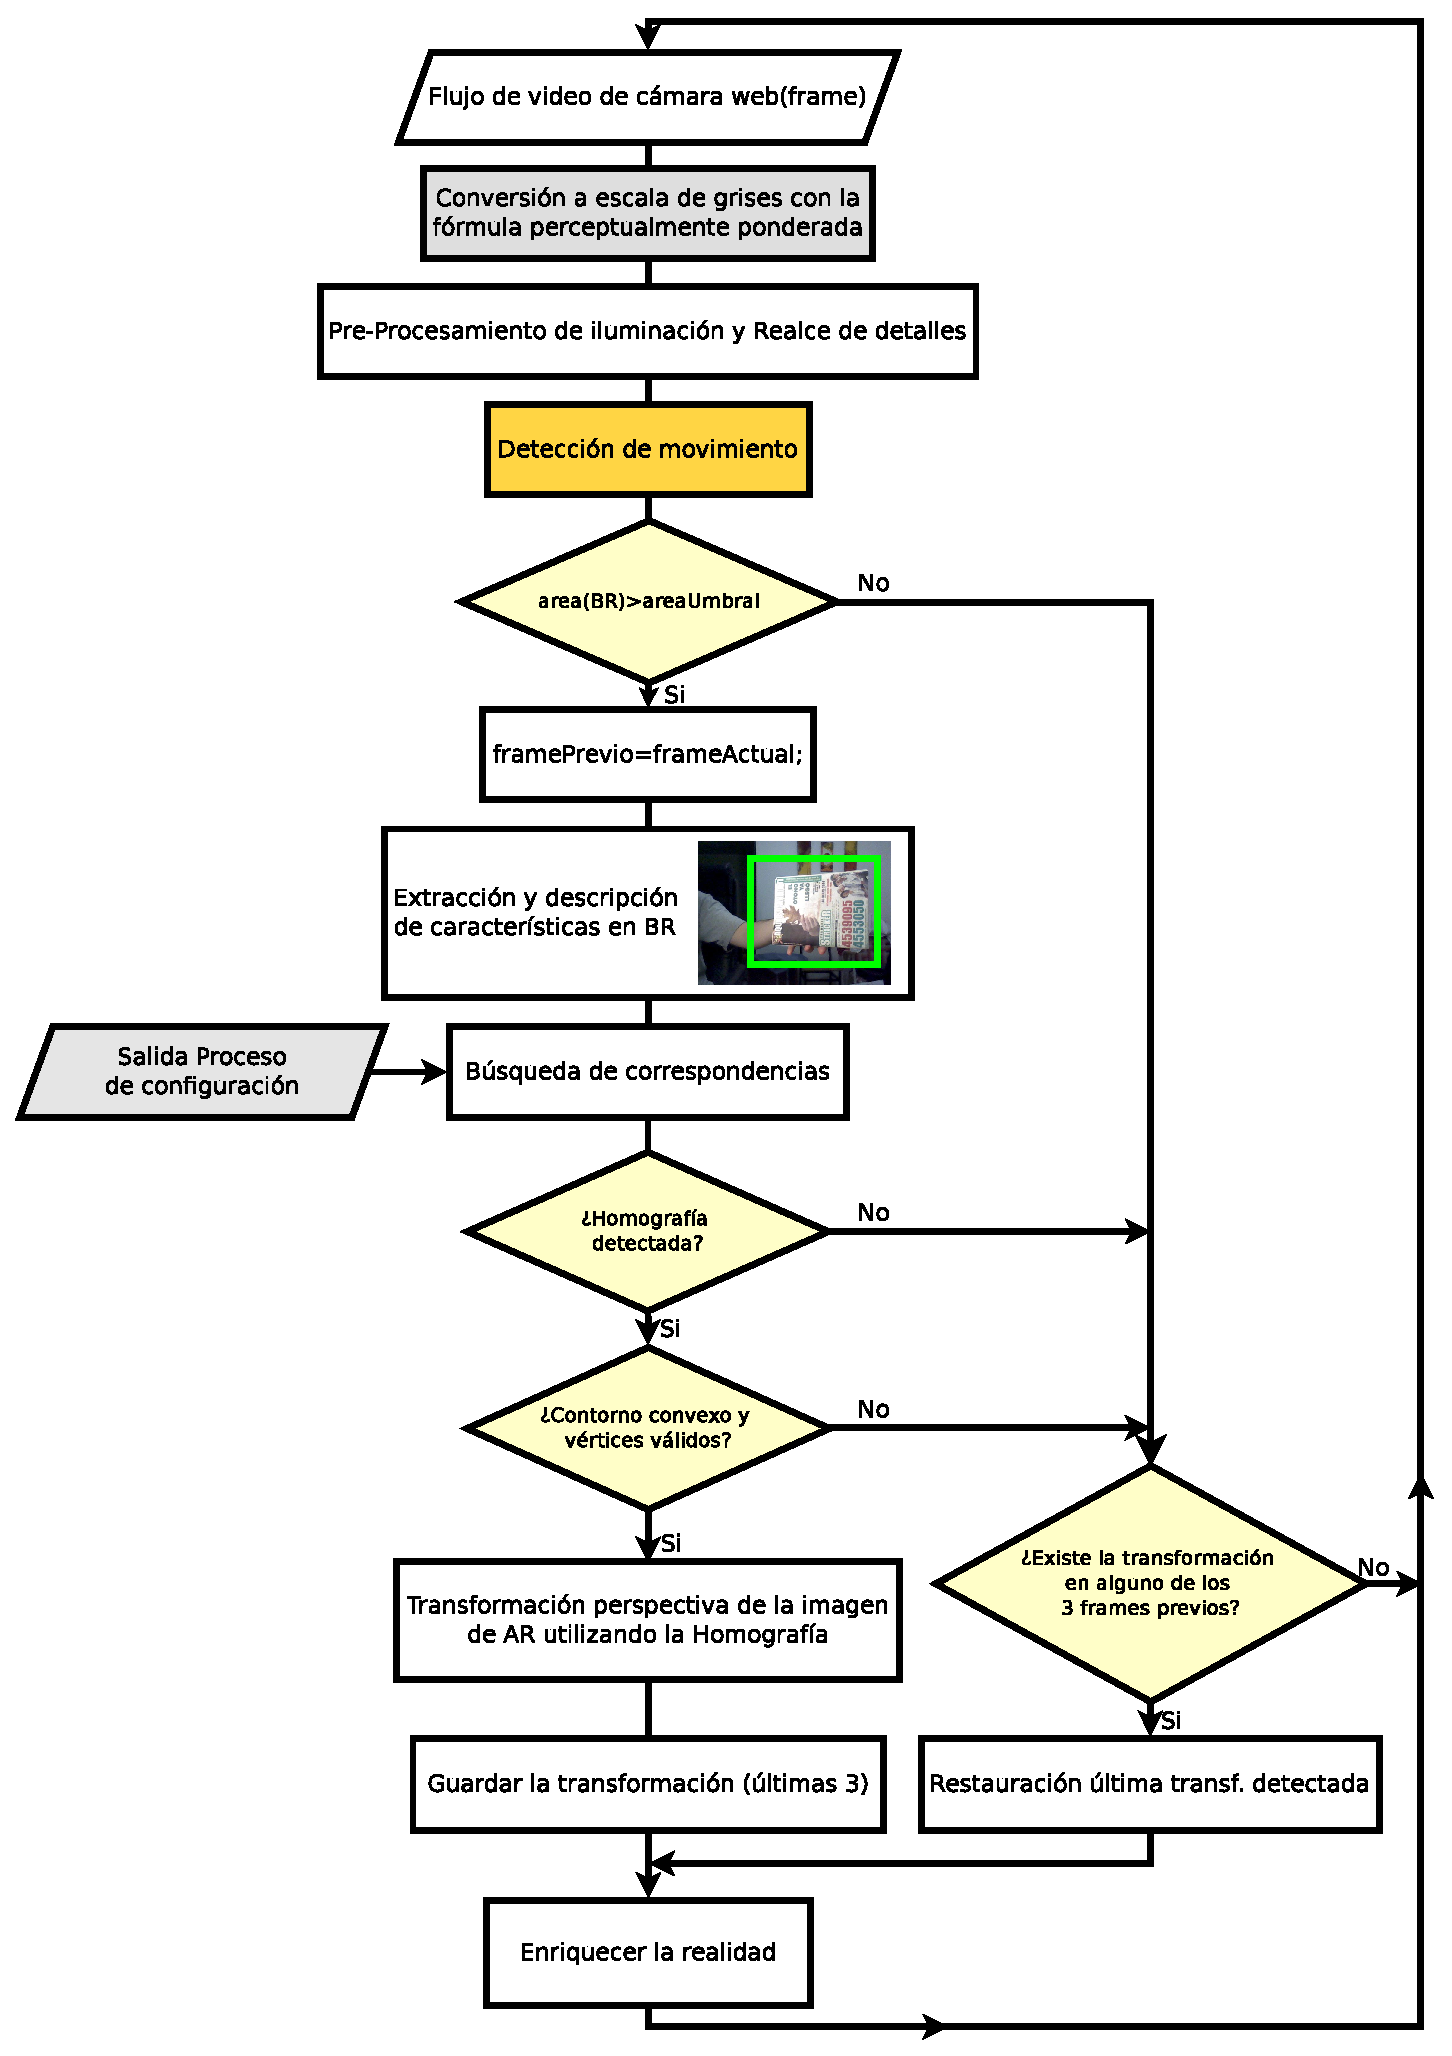
\includegraphics[scale=0.57]{../figs/proceso_completo}
    \caption[Diagrama de flujo de la etapa de ejecución]{Diagrama de flujo de la etapa de ejecución del método propuesto.}
   \label{fig:diagrama_metodo}                %% Etiqueta para la figura entera
\end{figure}

En la fase de configuración, la imagen de un objeto conocido es convertida a escala de grises mediante una fórmula perceptualmente ponderada de la forma que se expresa en la Sec. \ref{subsec:conver_escala_grises}. Tras ello, se aplica un proceso para mejorar la iluminación y resaltar detalles con el objetivo de mejorar la cantidad de puntos detectados, sobre todo en los casos en que la iluminación es baja. Luego, se procede con el método para la detección de características para obtener los puntos junto con sus descriptores asociados. Este proceso, tiene como salida un vector característico asociado a cada punto clave detectado, y es utilizado en la fase de ejecución para la detección del objeto.

En lo que respecta a la fase de ejecución, se aplica un proceso similar al anteriormente mencionado y se lleva a cabo sobre la imagen del flujo de video donde se busca el objeto. Un segundo paso consiste en utilizar los puntos claves y sus descriptores para la búsqueda de correspondencias de características. El proceso consiste en crear pares entre los descriptores de las imágenes pertenecientes a las dos fases mencionadas (configuración y ejecución) de acuerdo a sus similitudes, utilizando una búsqueda del vecino más cercano. Además, con el objetivo de aumentar la confianza respecto a los pares de correspondencias, se aplica un paso de eliminación de pares irrelevantes o espurios. Una vez que se obtiene un conjunto de correspondencias filtradas y potencialmente válidas, se estima la homografía con la ayuda de un método estadístico que le provee mayor confiabilidad en los resultados. Mediante la homografía, se obtiene un mapeo perspectivo entre la imagen patrón y la imagen del flujo de video (imagen objetivo). La existencia de la misma, establece la localización de la imagen patrón en la imagen objetivo y también especifica la transformación perspectiva que existe entre ellas. A pesar de haber aplicado un proceso para eliminar valores espurios, se presentan casos en que siguen existiendo valores inválidos de correspondencias que conllevan a una mala estimación de la homografía. Por ello, se establece un criterio para el rechazo de homografías mal estimadas basado en la forma convexa del polígono formado por la proyección de las esquinas de la imagen patrón de forma similar a la propuesta en \cite{BenhimaneNGGNM08}.
% las esquinas proyectadas de la imagen patr{on y su centro debe esta rdetnro de la imagen objetivo
% El poligono formado por la proyecci{on de la esquinas de la imagen patron debe ser convexo

Cabe aclarar que la extracción y descripción de características mediante SURF, la búsqueda de correspondencias mediante árboles KD aleatorios y la estimación de la homografía mediante RANSAC fueron integrados en el diseño del método de forma similar a la realización en \cite{BenhimaneNGGNM08}.

A continuación se presentan en detalle los procesos representados en los bloques de la Fig. \ref{fig:diagrama_metodo}.
\section[Conversión a escala de grises]{Conversión a escala de grises con una fórmula perceptualmente ponderada}
\label{subsec:conver_escala_grises}
Una imagen puede poseer varios canales de colores. En el caso del presente proyecto, la imagen que proviene del flujo de video es una imagen de tres canales (RGB). Debido a que el algoritmo utilizado para la extracción de características utiliza imágenes en tonos de grises de 8 bits, se aplica una conversión antes de procesar la imagen.

%La conversión a escala de grises, convierte la imagen de un espacio de color a otro, en este caso se convierte del espacio de colores RGB a escala de grises. 
Para el cálculo del valor de gris se usa la fórmula perceptualmente ponderada definida en la ecuación \eqref{eq:formula_conv_grises} donde $R$, $G$ y $B$ representan los canales rojo, verde y azul de la imagen de entrada respectivamente, e $I$ representa la imagen resultado convertida a tonos de grises:% (0 a 255 valores de intensidad).
\begin{equation}
\label{eq:formula_conv_grises}
I=0.299R+0.587G+0.114B.
\end{equation}
% Cabe aclarar, que se optó por trabajar con escalas de grises ya que esto implica menores tiempos de cálculos en los procesos y el método de extracción de características trabaja solo con imágenes de estas cualidades. 
\section{Mejoras en la iluminación y realce de detalles}
\label{sec:mejoras_ilum_detalles_metodo}
Como se ha mencionado el algoritmo SURF utilizado para la extracción y descripción de características, resulta variante a cambios de iluminación. Debido a ello, se plantean alternativas para aumentar el contraste de la imagen. Además, se ha notado un efecto de borroneado y/o detección de puntos insuficientes sobre todo en situaciones con imágenes en condición de iluminación baja, por lo que se han planteado algunas posibles estrategias para tratar de contrarrestar dicho problema.

Para esta etapa (``Pre-Procesamiento de iluminación y realce de detalles'' en la Fig. \ref{fig:diagrama_metodo}) se plantearon algunas alternativas simples de procesamiento en el dominio espacial: transformación logarítmica, ecualización de histograma, filtrado con pasa altos, filtrado de alta potencia y una combinación de ecualización y posteriormente filtrado de alta potencia. La elección de éstas técnicas se fundamentó principalmente en su velocidad de cómputo. La discusión de los resultados será presentada en la sección \ref{subsec:paraqumetros_utilizados}.
\section{Detección de la región de interés}
\label{sec:deteccion_cambiante_imagen}
En esta sección, se proponen algunos procesos orientados a obtener un menor tiempo de procesamiento y consecuentemente un menor tiempo de ejecución.

% Transformación de imágenes con operaciones morfológicas:
% Los filtros morfológicos, definen operaciones que transforman imágenes mediante la aplicación de elementos con formas predefinidas. La forma en que estos elementos intersectan la vecinidad de un pixel, determina el resultado de la operación.
Como es sabido, tanto el uso del método SURF para la extracción de ca-racterísticas como la búsqueda de coincidencias entre imágenes, conllevan un gran tiempo de procesamiento, el cual se convierte en un factor clave a la hora de lograr fluidez en la reproducción del flujo de video \cite{citeulike:9456628, Beis:1997:SIU:794189.794431, Friedman:1977:AFB:355744.355745, Liu04aninvestigation}. Para ata-car este problema, se propone detectar la región de interés (parte cambiante del flujo de video) y así aplicar el procesamiento sólo a una región de la imagen capturada. Para ello, se utilizan diferentes técnicas de procesamiento de imágenes en el siguiente orden: diferencia de imágenes, umbral, erosión, dilatación y detección del rectángulo delimitador mínimo. Estas herramientas, fueron elegidas debido a su simplicidad y al bajo tiempo de procesamiento que requieren, para no incrementar significativamente el tiempo de proceso total del algoritmo.

% \subsection{Detección de movimiento}
% \label{subsec:det_mov}
El objetivo es entonces, detectar la parte cambiante de la imagen entre un ciclo y el siguiente para realizar la extracción de características en la zona de la escena que ha cambiado, asumiéndose un sistema en el que la cámara web se encuentra fija y lo que se mueve es el objeto en la escena. Para esto, se llevan a cabo una serie de pasos que se observan en la Fig. \ref{fig:diagrama_procesomovimiento}, a fin de determinar un área que contenga el cambio de la imagen. A continuación, se describen cada una de las operaciones realizadas, cuyos resultados parciales pueden verse en la Fig. \ref{fig:deteccion_movimiento}.
\begin{figure}[tbhp]
   \centering
        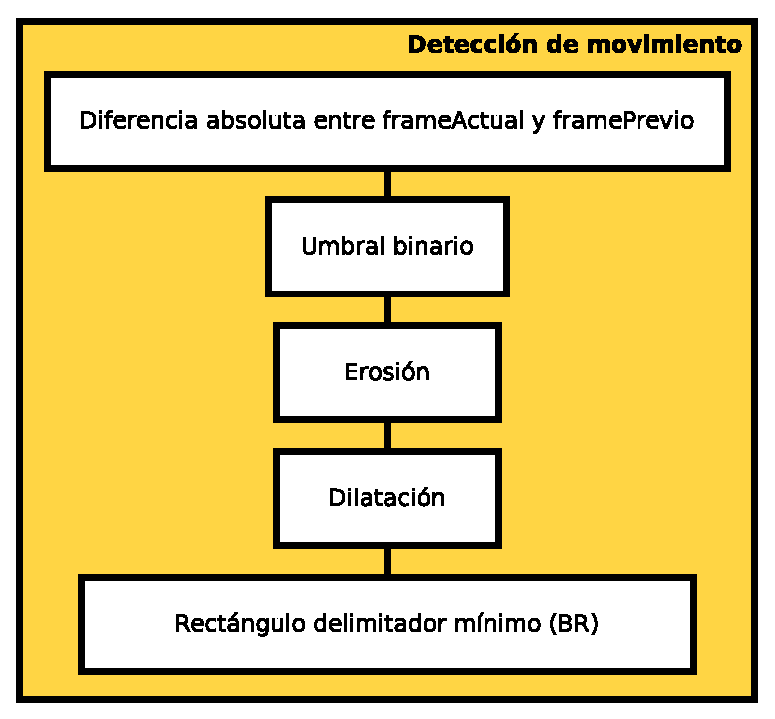
\includegraphics[scale=0.65]{../figs/procesomovimiento}
    \caption[Detalle del proceso de detección de movimiento]{Detalle del proceso de detección de movimiento introducido en el diagrama \ref{fig:diagrama_metodo}.}
   \label{fig:diagrama_procesomovimiento}                %% Etiqueta para la figura entera
\end{figure}
\begin{figure}[tbhp]
\centering
\subfloat[][Frame Previo]{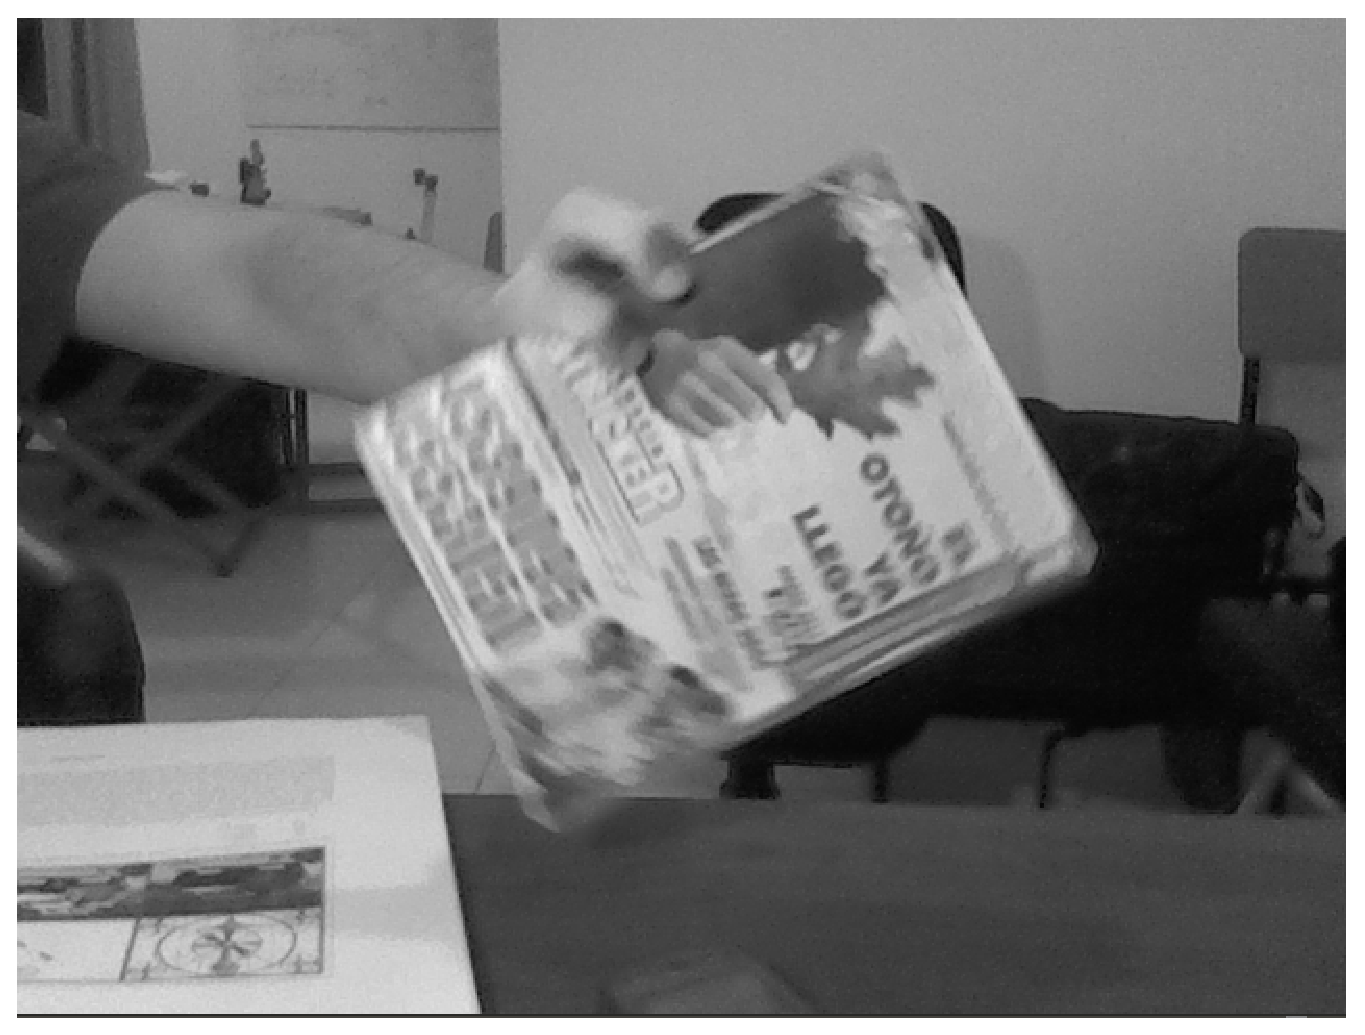
\includegraphics[width=2.3in]{../figs/preprocess/srcPrev} \label{fig:deteccion_movimietno-srcprev}}
\subfloat[][Frame Actual]{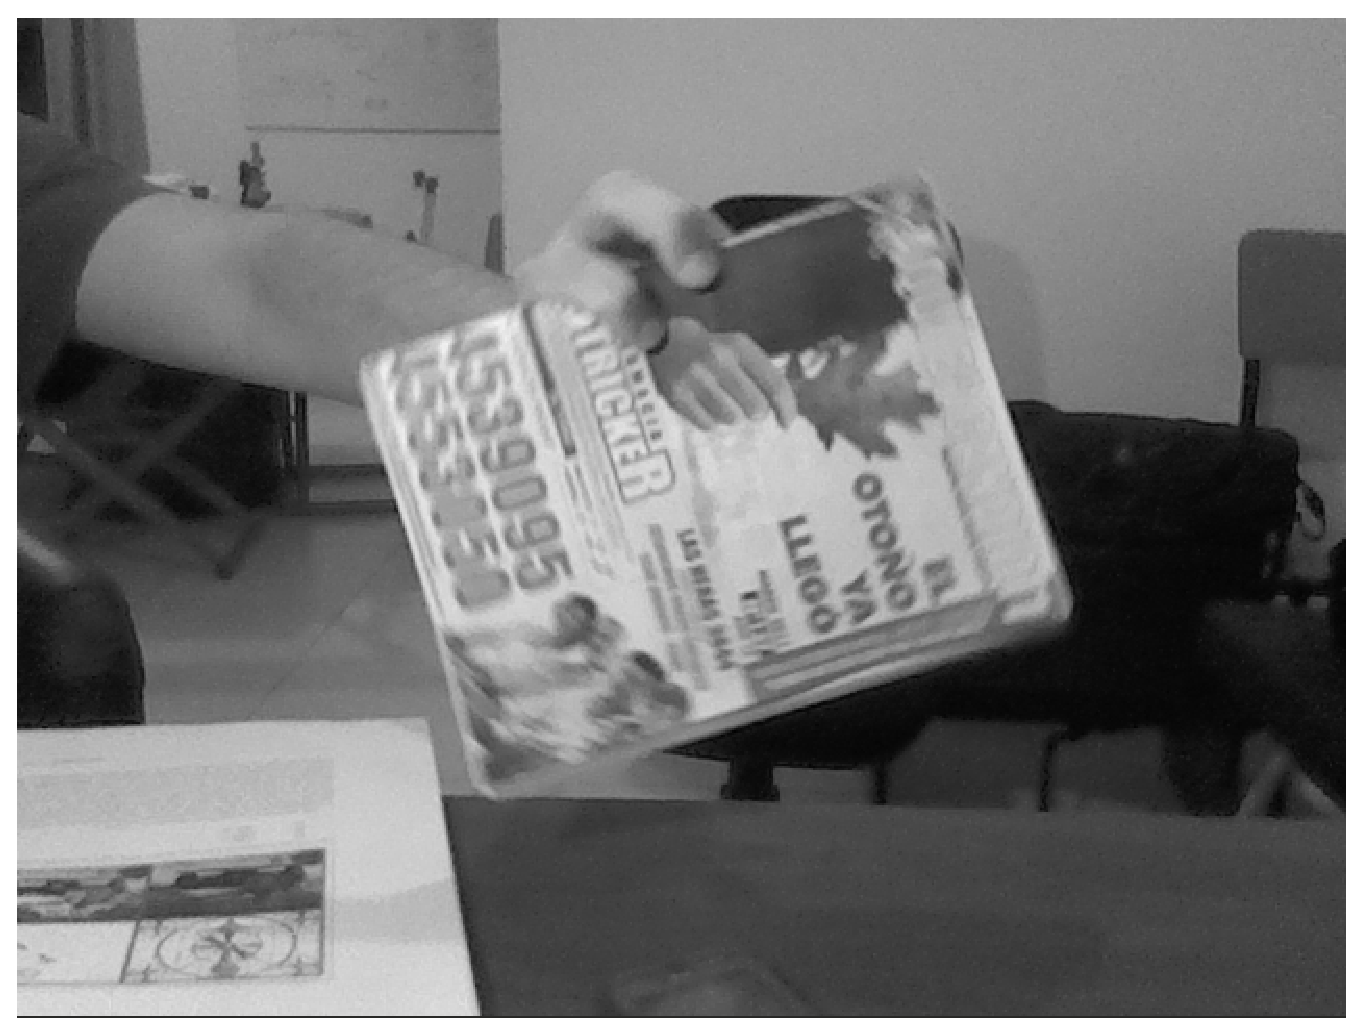
\includegraphics[width=2.3in]{../figs/preprocess/src} \label{fig:deteccion_movimietno-src}}\\
\subfloat[][Diferencia absoluta]{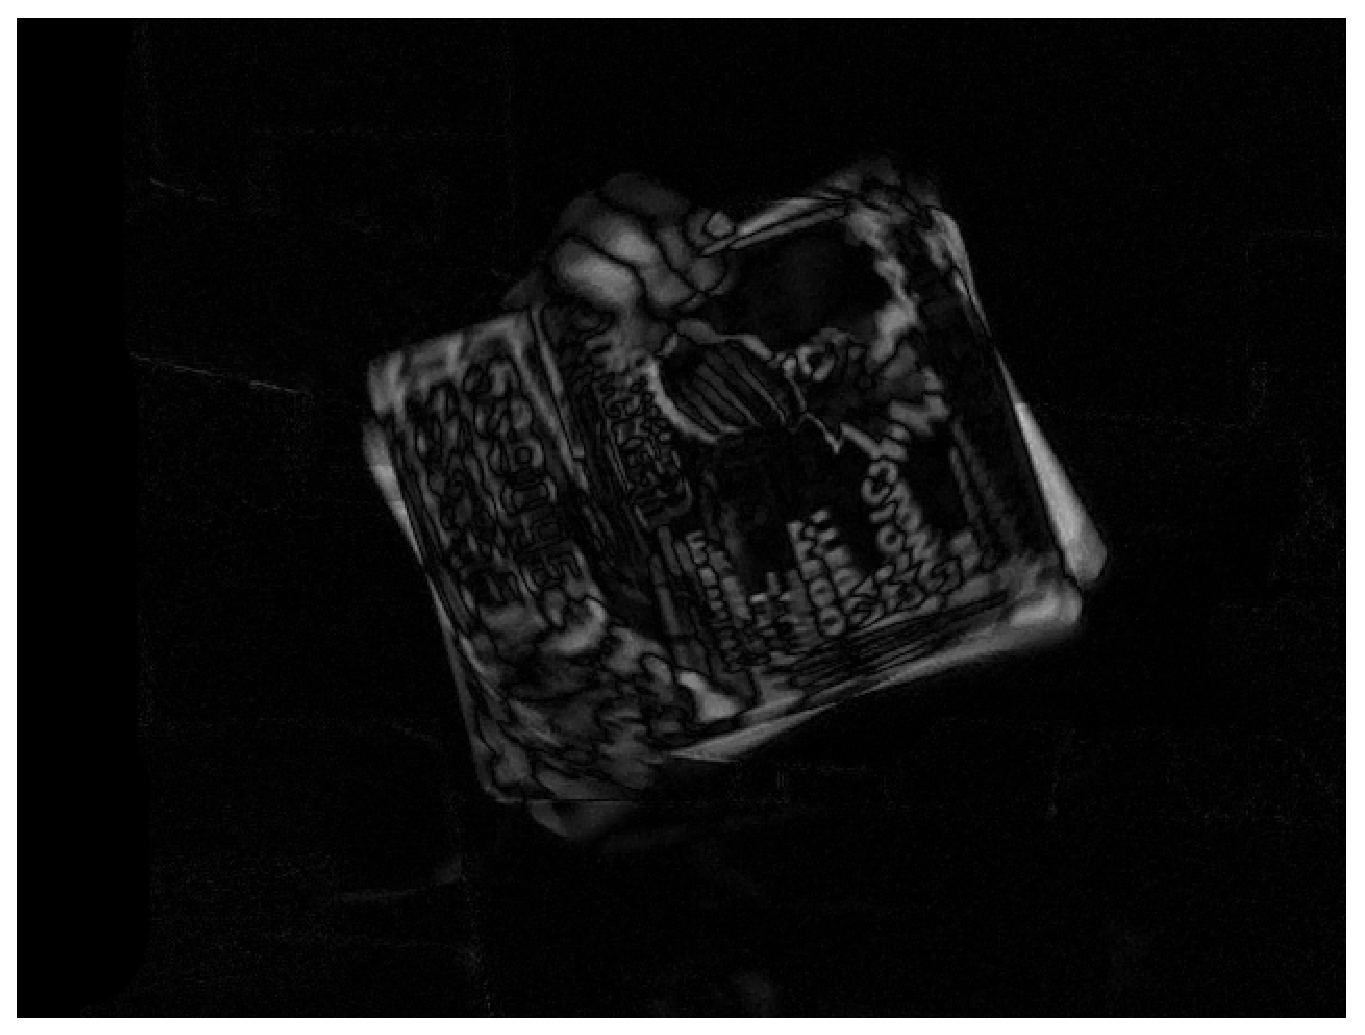
\includegraphics[width=2.3in]{../figs/preprocess/absDiff} \label{fig:deteccion_movimietno-absdiff}}
\subfloat[][Umbral binario]{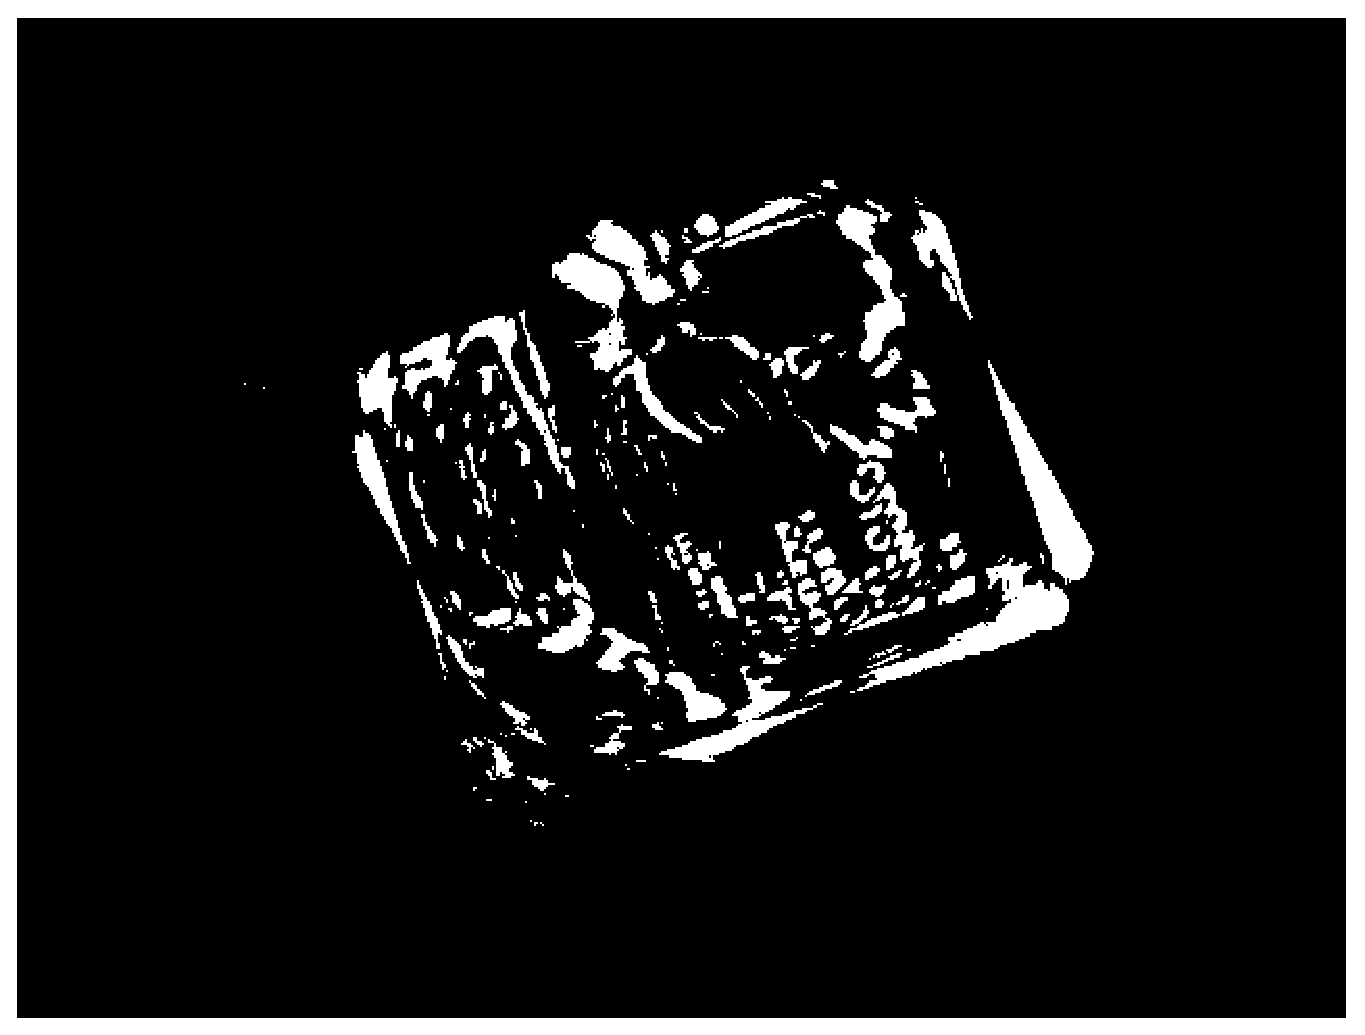
\includegraphics[width=2.3in]{../figs/preprocess/threshold} \label{fig:deteccion_movimietno-umbral}}\\
\subfloat[][Erosión $\times2$]{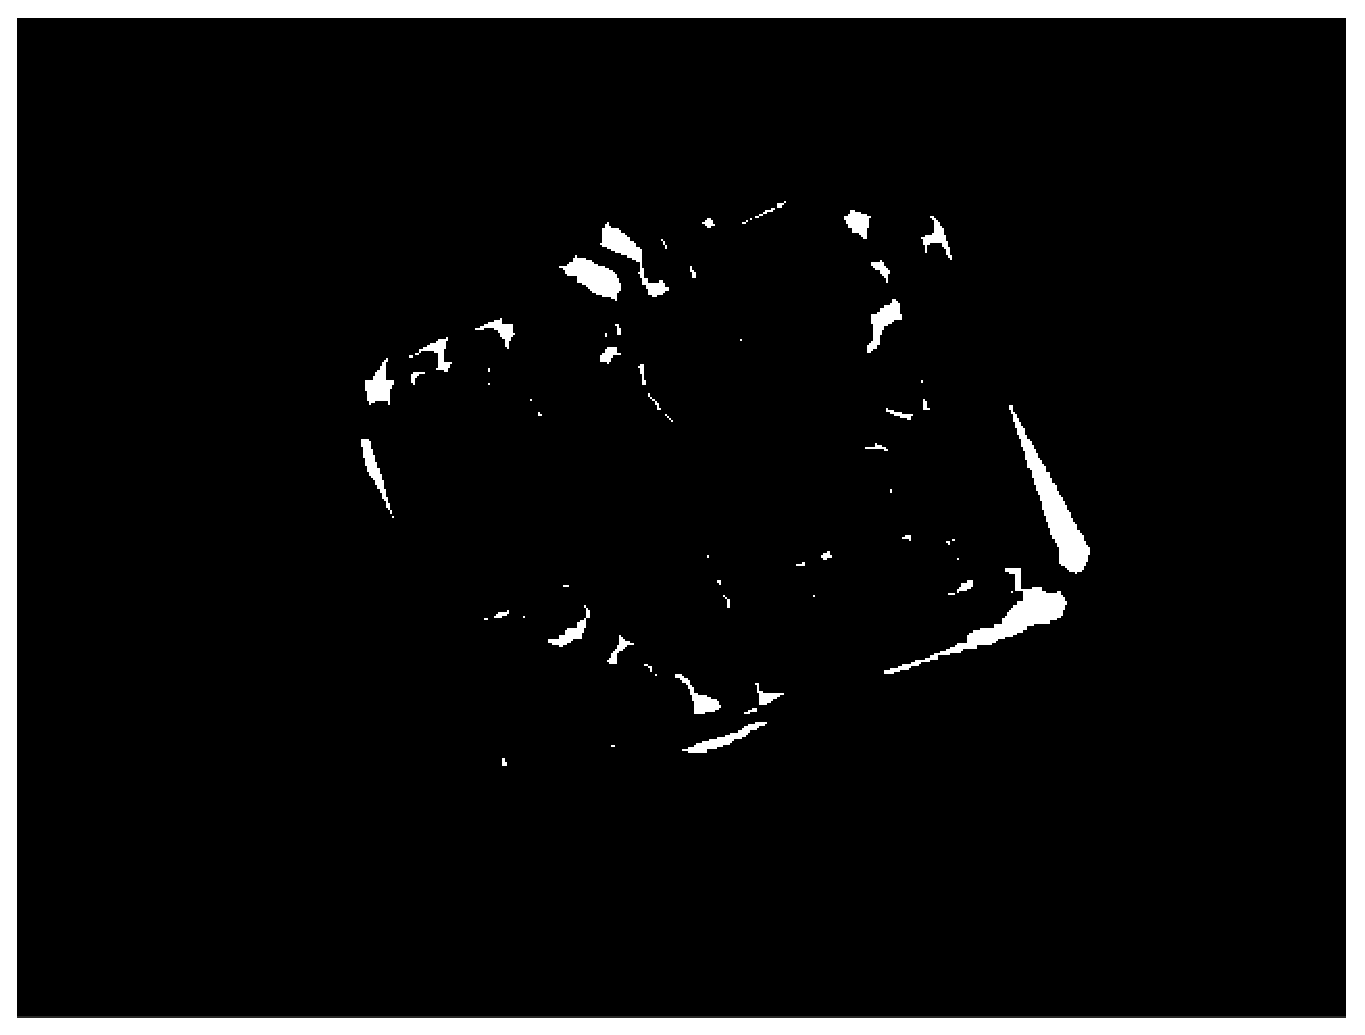
\includegraphics[width=2.3in]{../figs/preprocess/erode} \label{fig:deteccion_movimietno-erode}}
\subfloat[][Dilatación $\times2$]{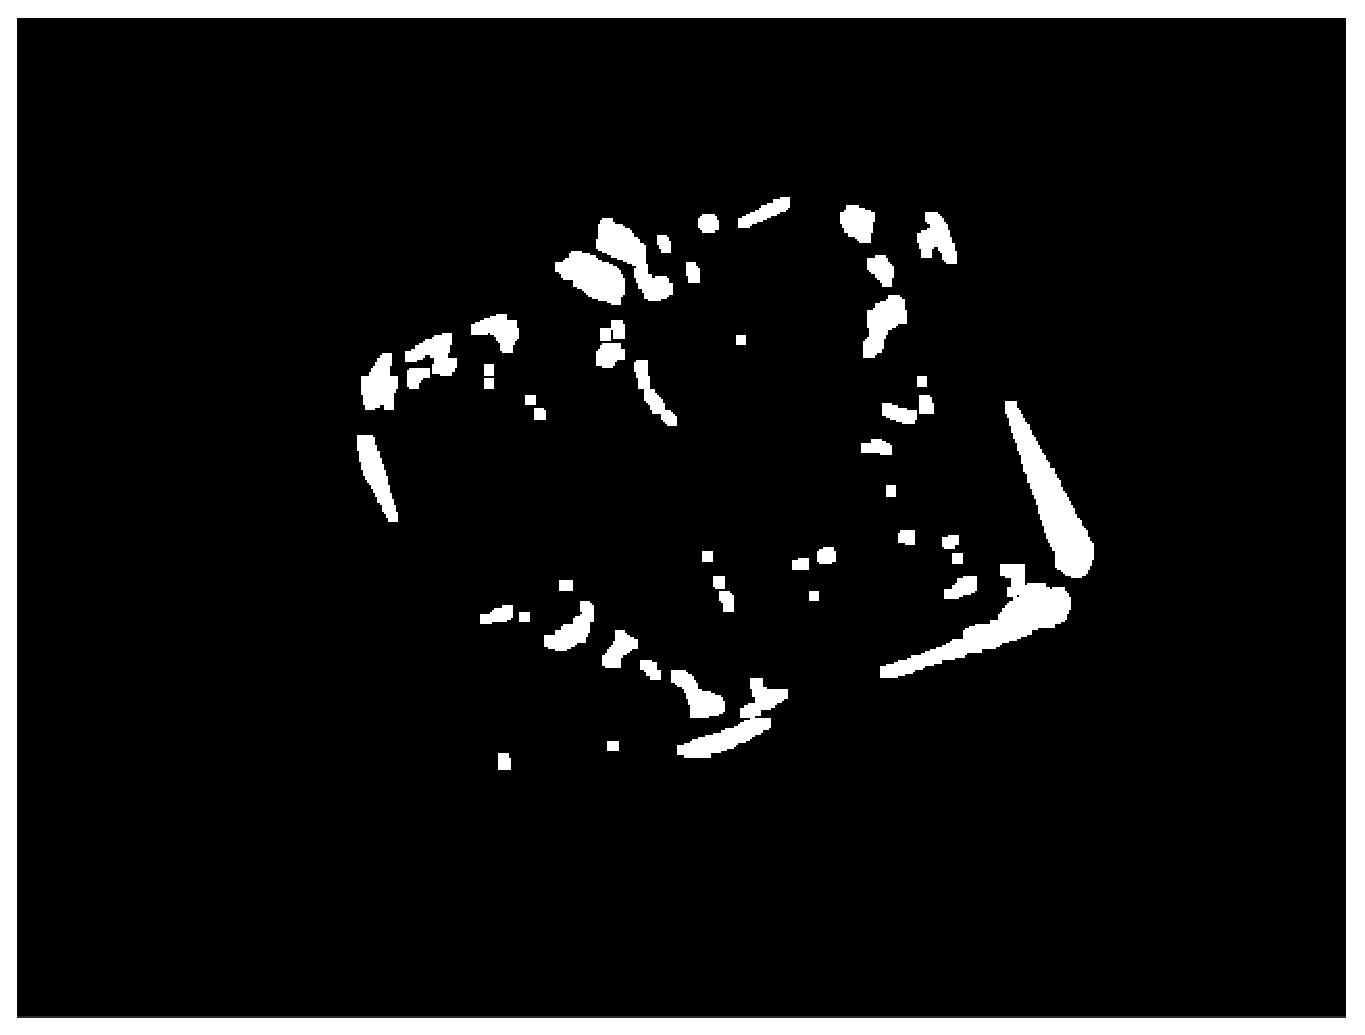
\includegraphics[width=2.3in]{../figs/preprocess/dilate} \label{fig:deteccion_movimietno-dilate}}\\
\subfloat[][Rectángulo delimitador mínimo]{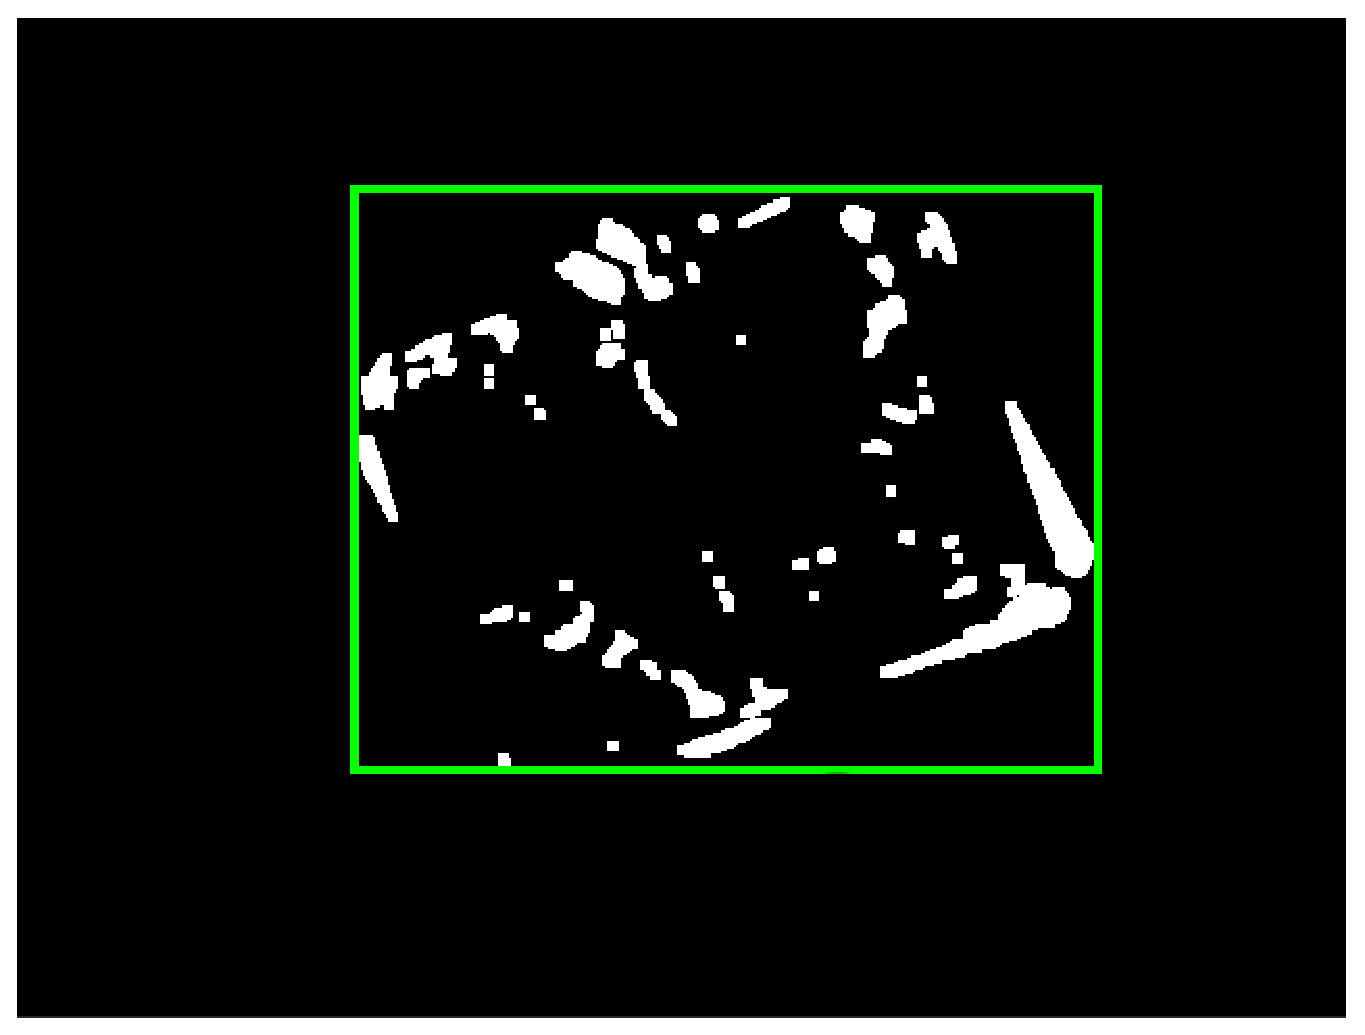
\includegraphics[width=2.3in]{../figs/preprocess/boundingrect} \label{fig:deteccion_movimietno-boundingrect}}
\caption[Detección de movimiento]{Resultado de los procesos aplicados para la detección de movimiento.}
\label{fig:deteccion_movimiento}               %% Etiqueta para la figura entera
\end{figure}
\subsubsection{Diferencia absoluta entre el frame actual y el frame previo}
La diferencia de imágenes es utilizada en el estudio del movimiento para detectar el cambio producido entre imágenes captadas en instantes de tiempo diferentes. Aquí se aplica con el objetivo de distinguir el cambio en la imagen cuadro a cuadro, y consiste en calcular el valor absoluto de la diferencia entre el cuadro $F$ del flujo de video capturado en el tiempo $t$ (actual) Fig. \ref{fig:deteccion_movimietno-src} y el capturado en $t-1$ (anterior) Fig. \ref{fig:deteccion_movimietno-srcprev}:
\begin{equation}
D(x,y)=|F_{t}(x,y)-F_{t-1}(x,y)|\;\forall\; x,y\;\in F.
\label{eq:diferencia_absoluta}
\end{equation}

El resultado de la operación es una imagen $D$ (Fig. \ref{fig:deteccion_movimietno-absdiff}) en la que se observa la parte que ha cambiado de una imagen a otra. Cabe aclarar que se utiliza el valor absoluto de la diferencia, ya que usar la resta produce resultados fuera del rango de valores que se utilizan en las imágenes. %En la Fig. \ref{fig:resta_invalida} se representa un ejemplo básico que muestra el resultado de la resta de dos frames de 8 bits con y sin valor absoluto (Fig. \ref{fig:resta_invalida} derecha e izquierda respectivamente). Los números en la Fig. \ref{fig:resta_invalida} indican el nivel de intensidad de los píxeles (0 para negro y 255 para blanco). Claramente se puede apreciar que no existe evidencia de cambio (el valor -255 se convierte a 0 en la imagen de 8 bits) en el caso de realizar la resta sin el valor absoluto, lo cual es incorrecto para la aplicación. %El color blanco en el resultado refleja la zona cambiante en la imagen.

% \begin{figure}[tbhp]
%        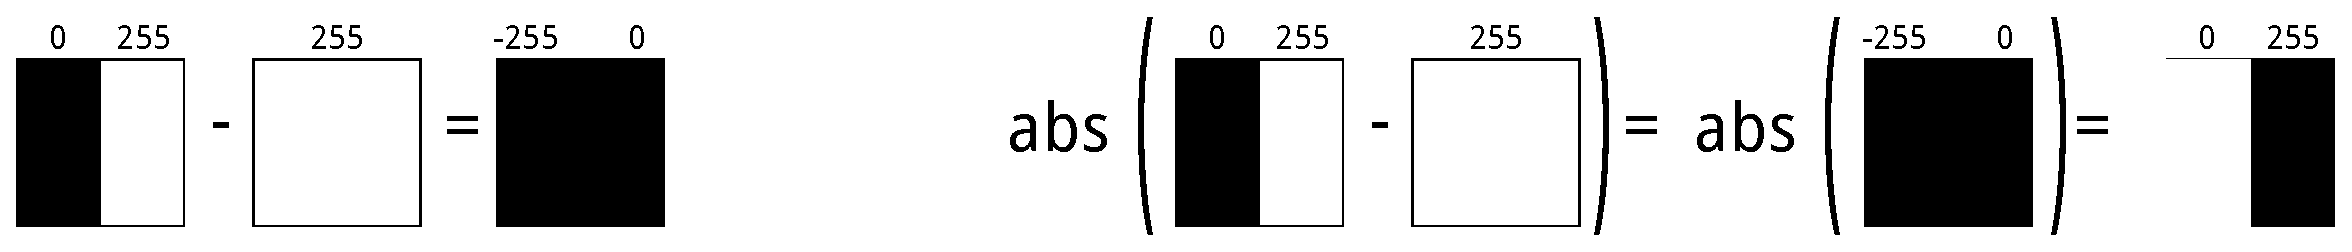
\includegraphics[scale=0.3]{../figs/restainvalida.eps}
%     \caption[Ejemplo de diferencia vs. diferencia absoluta entre frames]{Esquema ejemplo de diferencia vs. diferencia absoluta entre frames.}
%    \label{fig:resta_invalida}                %% Etiqueta para la figura entera
% \end{figure}
%%%%%%%%%%%%%%%%%%%%%%%%%%%%%%%%%%
Si bien se utiliza la ecuación \eqref{eq:diferencia_absoluta} para la diferencia de imágenes, el ``frame anterior'' no representa siempre el previo al actual procesado (nótese la asignación $framePrevio=frameActual$ dentro del condicional $area(BR)>areaUmbral$ en la Fig. \ref{fig:diagrama_metodo}). Es decir que la diferencia, se hace entre el fotograma actual y el último en el que se detectó movimiento. %Se tomó esta decisión, ya que si se realizaba la resta entre el actual y el efectivamente anterior capturado, ante pequeños o muy lentos movimientos del objeto en la escena, no se detectaba cambio alguno entre las imágenes (como consecuencia de las acciones que se describirán a continuación en esta sección), por lo que el objeto virtual dibujado en la escena quedaba mal dibujado.
Esta decisión, se ve fundamentada en el hecho que la diferencia entre frames sucesivos, donde el desplazamiento es muy pequeño, genera información espuria. Cabe agregar que ésto también beneficia al tiempo promedio de operación del sistema, ya que se ignora el cómputo de frames irrelevantes para la aplicación.

%no permite detectar movimiento en realidad..

% Si el objeto en la escena era rotado muy lentamente, no se alcanzaba a detectar el movimiento debido a que las acciones subsiguiente terminaban eliminando. Lo que se intento hacer es hacer la resta entre el frame actual y el previo, si no se detecta cambio se hace la diferencia entre el frame actual y el frame más viejo sobre el cual no se detectó un cambio en su momento. Una vez que se detecta el cambio, se empieza nuevamente con el mismo procedimiento. El efecto de esto no es visible cuando lo que se sobreimpone es una imágen, pero si se vería reflejado en el caso de un video por ejemplo ya que los frames procesados por segundo serían mayores caundo no hay movimiento de la imagen.
%%%%%%%%%%%%%%%%%%%%%%%%%%%%%%%%%%
Como se puede observar en la Fig. \ref{fig:deteccion_movimietno-absdiff}, existe presencia de ruido y ``patrones speckle'' en partes de la imagen donde no hay movimiento. Estos efectos indeseados, se tratarán de eliminar mediante una combinación de técnicas que se describen a continuación.
\subsubsection{Umbral Binario}
\label{subsub_ymbral}
A partir de la imagen diferencia $D$ obtenida anteriormente, se procede con la aplicación de un umbral binario de la forma que se expresó en la ecuación \eqref{eq:equation_umbral_binario} para remover valores de intensidad bajos (ruido y ``patrones speckle'' pueden ser observados debajo de la esquina inferior izquierda de la revista en la Fig. \ref{fig:deteccion_movimietno-absdiff}). Se asigna el valor $s_{max}=255$ a los píxeles que superen el umbral con un valor definido empíricamente ($u=50$) y $0$ a los demás píxeles, obteniéndose como resultado una nueva imagen $s$, ver Fig. \ref{fig:deteccion_movimietno-umbral}.

A pesar de haber eliminado gran parte del ruido en la imagen, en la práctica se dan casos en los que puntos aislados continúan apareciendo en la imagen. Variar el límite ($u$) establecido para la umbralización no brinda una solución a este problema, ya que al aumentar $u$ se elimina información importante y al disminuirlo, aumenta la información espuria. Es por esto que fue necesario proponer dos procesos que se mencionan a continuación.
%Se intentó aumentar el límite de $u$, pero esto derivó en la pérdida de otros puntos que resultaban de interés para el análisis, por lo que se decidió dejar este valor establecido de forma que el mismo garantice mantener las zonas que resulten de interés para el análisis y se aplicaron 2 acciones que se mencionan a continuación para lograr eliminar los puntos aislados.
\subsubsection{Erosión y dilatación}
Para eliminar los puntos aislados que no hayan sido removidos anteriormente, se propone aplicar una operación de erosión. Posteriormente, se aplica una operación de dilatación para recuperar el tamaño aproximado de los objetos de interés.
% mientras que la dilatación se aplica para no perder el análisis en áreas en que ha ocurrido movimiento las cuales han sido eliminadas, en parte, debido a la operación de erosión anteriormente mencionada.

Para llevar a cabo la erosión y la dilatación, se utilizó un kernel de $3 \times 3$ píxeles y cada una de las operaciones fue aplicada dos veces (dos erosiones y luego 2 dilataciones). En el caso que haya habido movimiento, el resultado final es una imagen negra con un sector blanco, que representa la zona cambiante de la imagen. El resultado se puede observar en la Fig. \ref{fig:deteccion_movimietno-erode} y \ref{fig:deteccion_movimietno-dilate}.
% Una buena forma de ver el efecto de este operador es en términos de una imagen con fondo negro y objetos blancos. Cuando se aplica la erosión, si un píxel del filtro aplicado esta sobre el fondo, luego el pixel sobre el cuál se esta aplicando la erosión resultará con el valor del fondo. Mientras, que en el caso de la dilatación, si el filtro toca un objeto sobre el fodno, el pixel será asignado al valor del blanco. 
% poner que máscara se usa y poner imagen
% cvErode(frameDiferencia, frameDiferencia, NULL, 2);
% cvDilate(frameDiferencia, frameDiferencia, NULL, 2);
%http://opencv.willowgarage.com/documentation/miscellaneous_image_transformations.html?highlight=cvthreshold#cvThreshold
\subsubsection{Rectángulo delimitador mínimo}
\label{subsubsec:bounding_rect}
En este paso se busca detectar el rectángulo más pequeño que encierra a todos los puntos cuyo valor no es negro. Al utilizar un rectángulo delimitador mínimo (del inglés, bounding rect o BR), se pueden descartar regiones de la imagen que no necesitamos procesar en el algoritmo. %Debido que anteriormente hemos eliminado el ruido mediante las operaciones de umbral, dilatación y erosión, nos aseguramos de esta forma el poder encontrar un único rectángulo válido. 
%BR contendrá la parte cambiante de la imagen sobre la que detectaremos características y haremos el posterior proceso de correspondencia y detección de la ubicación de la imagen patrón. 
El resultado final de la operación se puede observar con un rectángulo de color verde en la Fig. \ref{fig:deteccion_movimietno-boundingrect}.
\subsection{Área del rectángulo delimitador mínimo}
\label{subsec:validacion_area_boundingrect}
La detección de la parte cambiante de la imagen en el flujo de video, determina un BR sobre el que se ejecuta el procesamiento. En la práctica, se pueden identificar situaciones particulares que involucran la determinación del BR:
\begin{enumerate}
 \item ¿Qué sucede si no se detecta movimiento?
 \item ¿Qué sucede si el BR del área detectada es demasiado pequeña?
\end{enumerate}

Para dar respuesta a estos interrogantes, se ha propuesto un proceso en el algoritmo que censa el tamaño del BR mediante un bloque condicional presentado en el diagrama de la Fig. \ref{fig:diagrama_metodo}, cuya expresión es: $area(BR)>areaUmbral$, donde $area(\cdot)$ es una función que calcula el área en píxeles sobre el argumento y $areaUmbral$ el valor en píxeles que el área debe superar.

Respecto al primer interrogante, si no existe movimiento tampoco existe $BR$ y por ende la condición de área no se satisface. Entonces, el flujo del procesamiento se deriva al procedimiento establecido en la Sec. \ref{subsubsec:presente_en_alguno_3_frames_previos}.

Para la segunda pregunta, se hizo una búsqueda del valor óptimo de $areaUmbral$ para la configuración general de la escena que se utiliza. El mismo fue establecido de manera empírica en $10000$ píxeles que fue el valor con el que se obtuvieron mejores resultados. Ésto limita la detección cuando las esquinas proyectadas de la imagen patrón resultantes de aplicar la homografía, forman un área relativamente pequeña (se puede pensar en un cuadrilátero de $100 \times 100$ sobre la ventana de $640 \times 480$). Obtener la cantidad suficiente de características en objetos de estos tamaños es una limitante que presenta el dispositivo de adquisición de imágenes utilizado. De esta manera, si el área de BR no supera el umbral establecido, se considera a la región como ``demasiado pequeña'' y el procesamiento al igual que en el caso anterior, se deriva a la acción que se describe en la Sec. \ref{subsubsec:presente_en_alguno_3_frames_previos}.
%%%%%%%%%%%%%%%%%%%%%%%%%%%%%%%%%%%%%%%%%%%%%%%%%%%%%%%%%%%%5
\section{Extracción y descripción de características}
\label{sec:extract_y_descrip_caracteristicas}
En la etapa de extracción y descripción de características, se detectan puntos claves o de interés en la imagen que se está analizando con el método que se describió en la Sec. \ref{sec:detec_ptos_claves}. Dicha detección se realiza en la subimagen determinada por BR. % descripto en la Sec. \ref{subsubsec:bounding_rect}. 
Esta etapa involucra básicamente dos pasos:
\begin{enumerate}
 \item Detectar los puntos claves en la imagen.
 \item Extraer un vector de características (64 elementos) para cada punto detectado en la imagen.
\end{enumerate}
% 
% 1. Detect suitable keypoint features in the image
% 2. Extract a feature vector at each keypoint
% 3. Match the features
% 4. Filter out the bad matches
% 5. Perform pose estimation on the good matches
% http://experienceopencv.blogspot.com.ar/2011/01/surf-detector.html
% La extracción y descripción de características es realizada dentro del br.?

Para llevar a cabo dichos pasos, se ha utilizado un algoritmo descripto en \cite{Bay06surf:speeded} para el cual se especifican los siguientes parámetros: %algunos de los parámetros de entrada mencionados en la Sec. \ref{sec:detec_ptos_claves}:
\begin{itemize}
 \item \textbf{nOctaves}: identifica el número de octavas que se utilizan en la búsqueda de puntos claves. Se estableció en el valor 4 en el que se obtuvieron resultados satisfactorios \cite{Bay06surf:speeded}.
 \item \textbf{nOctaveLayers}: es el número de filtros o capas utilizado dentro de cada octava. Se estableció en el valor 3 ya que resultó adecuado y es recomendado en \cite{Bay06surf:speeded}.
 \item \textbf{hessianThreshold}: es un valor de umbral que se utiliza para eliminar máximos locales detectados con el determinante del hessiano descripto en la Sec. \ref{sec:detec_ptos_claves}. Aquellas características cuyo determinante del hessiano superan dicho umbral son extraídas. Los valores para este parámetro, dependen del promedio local del contraste, la nitidez y los detalles de la imagen. Estos valores serán tratados en el capítulo \ref{c:pruebas_resultados_discusion}. 
 Un ejemplo de los efectos de este parámetro sobre una misma imagen puede ser observado en las Fig. \ref{fig:extraccion800} y \ref{fig:extraccion3000}, donde la línea verde representa la orientación para el punto clave detectado (marcado en color azul) y la escala viene representada por el círculo rojo centrado en cada punto clave. En la Fig. \ref{fig:extraccion800} se fijó el umbral en 800 (más puntos detectados), mientras que en la Fig. \ref{fig:extraccion3000} se utilizó el valor 3000 con lo cual se puede ver una disminución en la cantidad de los puntos detectados.
\end{itemize}
% El valor utilizado para \textit{nOctaves} y \textit{nOctaveLayers}, se ha .
% Los puntos claves SURF son aquellos cuyos valor promedio de intensidad de los pixeles difieren ampliamente de sus inmediatos vecinos.
% Una vez que el descriptor SURF y sus puntos claves son calculados, estos pueden ser comparados usando uno o más algoritmos conocidos, como los son el de búsqueda del vecino más cercano (Nearest Neighbor Search), K-Means Clustering, etc. 
      \begin{figure}[tbhp]
	\centering
	%%----primera subfigura----
	\subfloat[]{
	      \label{fig:extraccion800}         %% Etiqueta para la primera subfigura
	      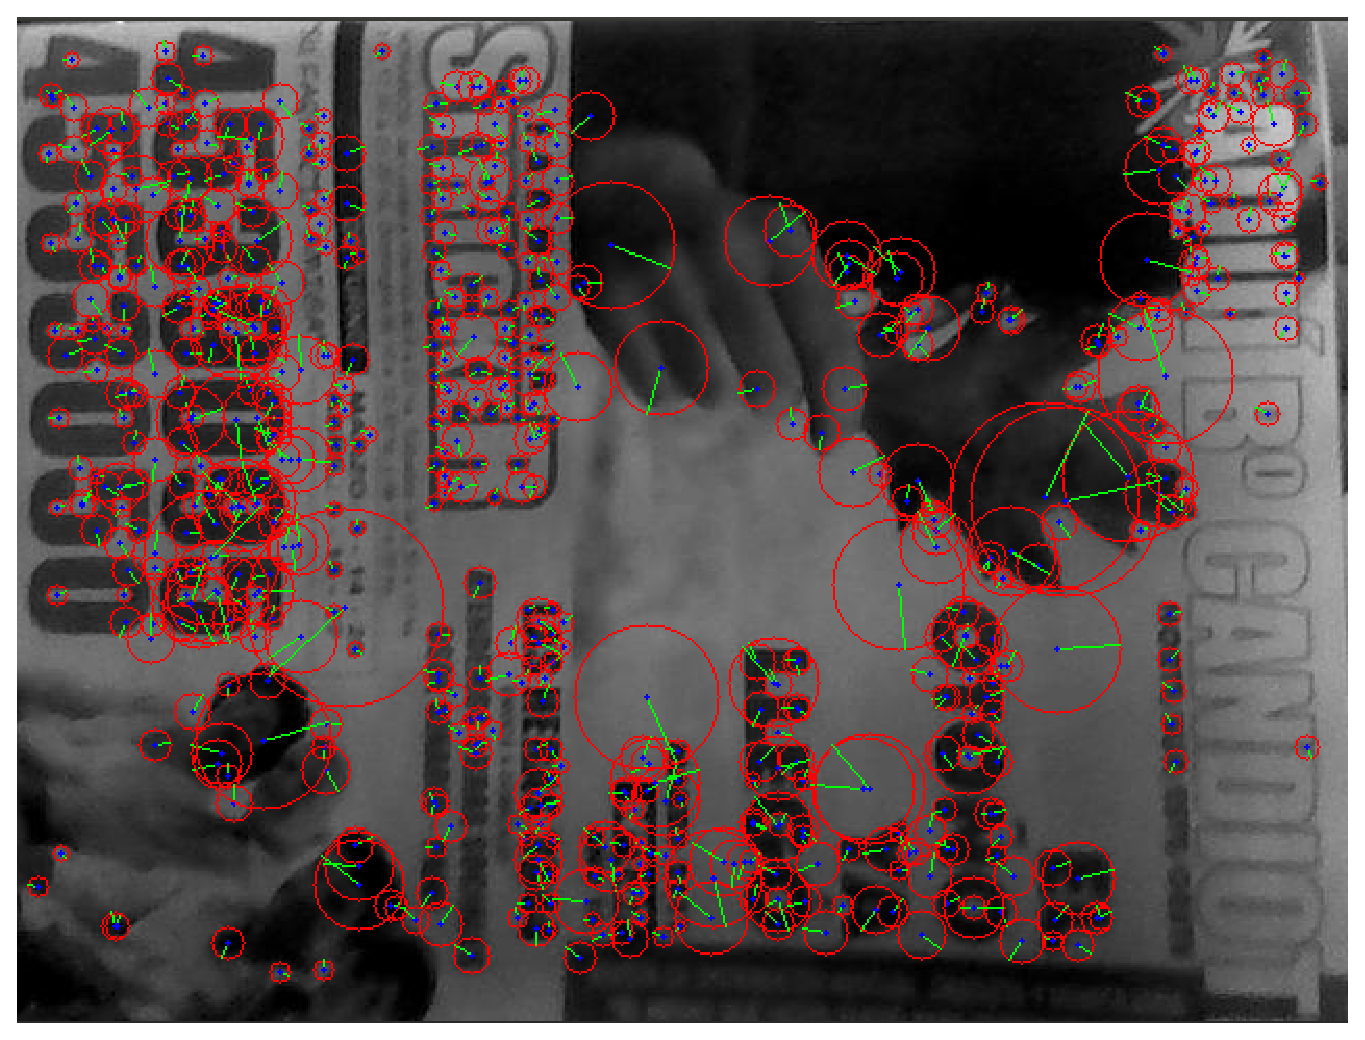
\includegraphics[scale=0.5]{./figs/extraccion/800}}
	\hspace{0.1\linewidth}
	%%----segunda subfigura----
	\subfloat[]{
	      \label{fig:extraccion3000}         %% Etiqueta para la segunda subfigura
	      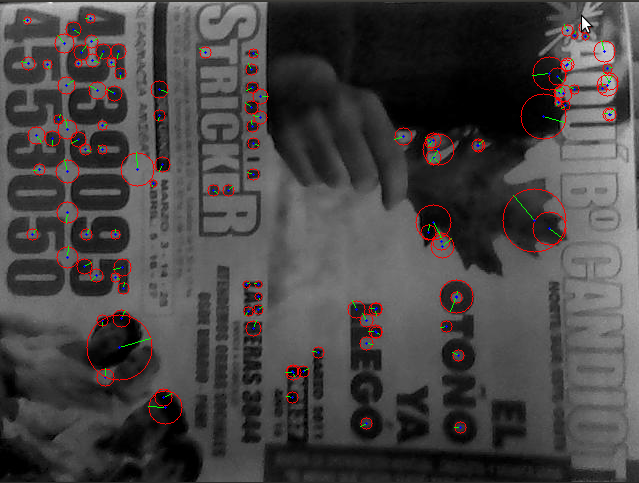
\includegraphics[scale=0.5]{./figs/extraccion/3000}
	  }
	\label{fig:extraccioncaracteristicas}                %% Etiqueta para la figura entera
	\caption[Ejemplo de extracción de características en una imagen]{Extracción de características para la imagen patrón con dos va-lores de umbral aplicado sobre el Hessiano.}
      \end{figure}
%%%%%%%%%%%%%%%%%%%%%%%%%%%%%%%%%%%%%%%
\section{Correspondencia entre puntos claves}
Luego de detectar los puntos claves y sus descriptores tanto en la imagen patrón como en la imagen objetivo, se procede con la búsqueda de coincidencias entre ambas imágenes. Para ello, se utiliza la búsqueda del vecino más cercano, aquí se utilizan dos vecinos al punto clave detectado como se describe en la sección \ref{sec:correspop_ptos_claves}. Además, se utiliza la técnica de árboles KD para acelerar la búsqueda y el filtrado de correspondencias no válidas, que se describió en la sección \ref{sec:remocion_corresp_invalidas}.

De esta forma se obtiene un conjunto de pares de puntos entre la ima-gen patrón y la imagen objetivo. Un ejemplo puede ser observado en la Fig. \ref{fig:correspondencias_deteccion_lineas}, donde los parámetros descriptos en la Sec. \ref{sec:remocion_corresp_invalidas} se establecieron a $\mathit{hessianThreshold}=2000$ y $\varepsilon=0.8$. Las líneas entre las imágenes representan las correspondencias detectadas entre los puntos claves de la imagen patrón (izquierda) y la imagen objetivo (derecha), correspondiente al flujo de video en un instante de tiempo. Las correspondencias espurias que se pueden observar (por ejemplo, la letra ``o'' en la palabra ``otoño''), pueden ser luego descartadas mediante el uso de RANSAC en la estimación de la homografía.
\begin{figure}[tbhp]
   \centering
        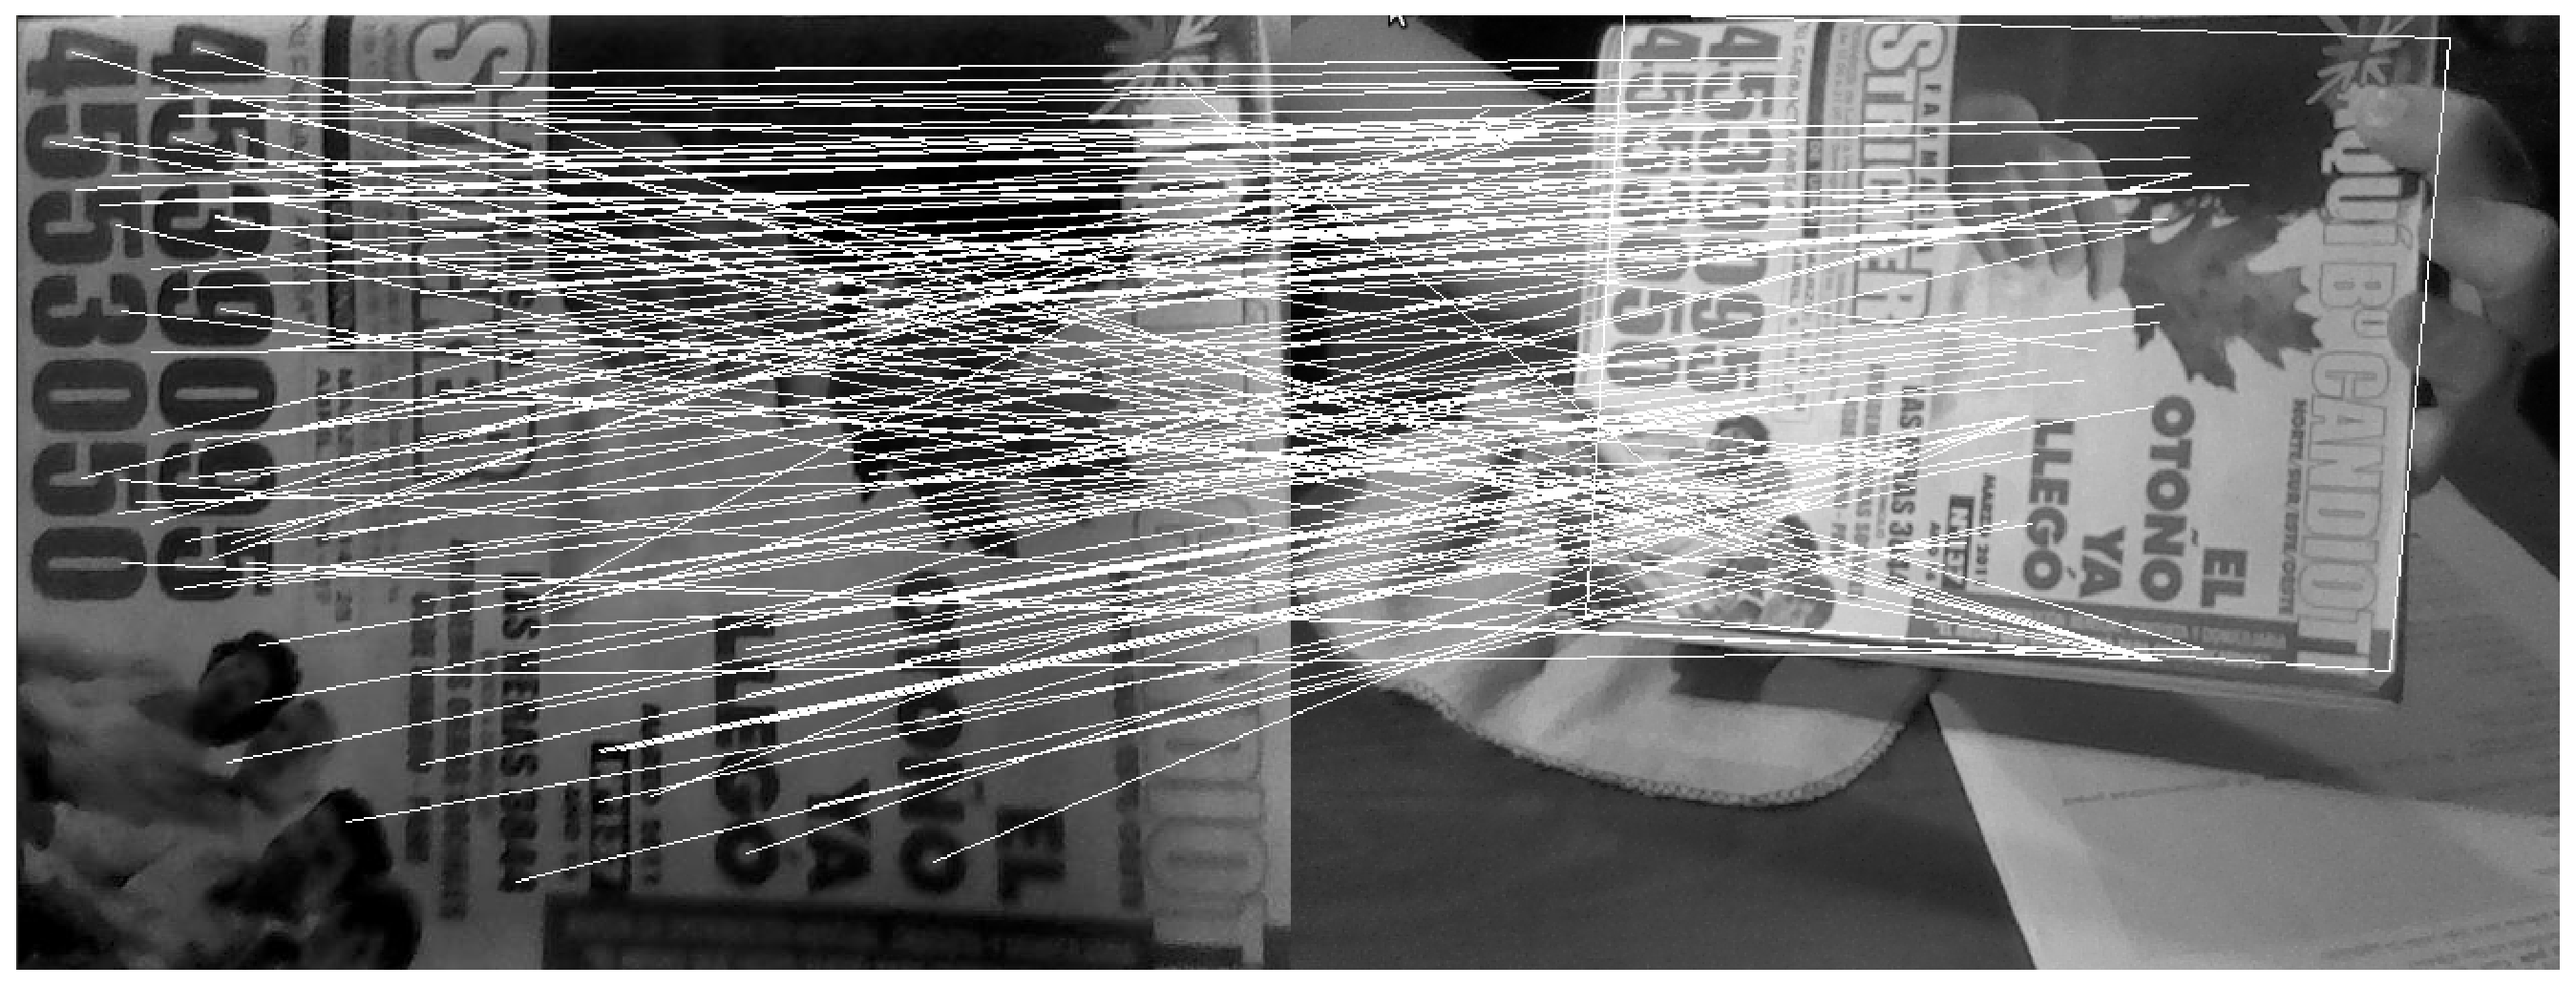
\includegraphics[scale=0.3]{../figs/extraccion/correspondencias}
    \caption[Correspondencias de puntos entre imágenes patrón y objetivo]{Correspondencias de puntos entre imágenes patrón y objetivo antes de estimar la homografía con RANSAC.}
   \label{fig:correspondencias_deteccion_lineas}                %% Etiqueta para la figura entera
\end{figure}

Las funcionalidades de búsqueda del vecino más cercano, junto con el armado de árboles para una indexación más rápida fueron realizadas mediante la interfase FLANN\footnote{\url{http://opencv.willowgarage.com/documentation/cpp/flann_fast_approximate_nearest_neighbor_search.html}} provista por OpenCV. %sobre la cual no se entró en detalle!??
%%%%%%%%%%%%%%%%%%%%%%%%%%%%%%%%%%%%%%%
\section{Detección de homografía}
\label{sec:detec_homografia}
La transformación proyectiva u homografía es la proyección perspectiva entre dos imágenes y es derivada de las posiciones de los puntos claves en la imagen patrón y los puntos coincidentes detectados en la imagen objetivo, de acuerdo a como se ha explicado en la Sec. \ref{sec:transf_proyectiva_homograph}. En este trabajo, la existencia de la homografía entre los puntos en la imagen patrón y los de la imagen objetivo significa que el objeto (representado por la imagen patrón) existe en la imagen objetivo.

Como se ha mencionado en la Sec. \ref{sec:estimacion_ransac_homografia}, existen diferentes opciones para llevar a cabo la estimación. En el presente trabajo, se usará el algoritmo RANSAC, ya que este brinda mejores resultados cuando hay varios puntos de correspondencia espurios, lo que es común en el caso de localizar objetos planos en la escena \cite{BenhimaneNGGNM08}. La desventaja de usar el algoritmo RANSAC recae en que, dados más de cuatro puntos, siempre se encuentra la homografía independientemente si ésta tiene sentido. Es decir, que si el objeto no se halla en la escena, pero se encuentran coincidencias que son espurias, la homografía será detectada y producirá resultados indeseables. %La homografía también captura las transformaciones, como el tamaño, localización y rotación del objeto en la escena.
% Las función utilizada para la estimación de la Homografía con RANSAC no fue implementada sino que se utilizó la provista por la librería OpenCV (cvFindHomography).
%%%%%%%%%%%%%%%%%%%%%%%%%%%
\section{Detección de homografías mal estimadas}
\label{sec:salvado_convexidad_vertices}
Para salvar los casos en que no se detecta el objeto o la transformación con la homografía hallada presenta una morfología inválida, se aplican algunas validaciones. Las alternativas que se proponen, han permitido obtener un mejor resultado en la detección del objeto en la imagen objetivo, eliminando los falsos positivos. Para ello se utilizan dos criterios:
\begin{itemize}
 \item Convexidad
 \item Distancia entre vértices
\end{itemize}
\subsubsection{Convexidad}
Este criterio es usado para rechazar transformaciones deformes que forman una figura cóncava incorrecta (forma de mariposa, véase la Fig. \ref{fig:poligono_concavo_invalido}). Consiste en comprobar la convexidad sobre el polígono formado por las esquinas proyectadas de la imagen patrón, luego de aplicar la transformación con la matriz de homografía. En el caso de polígonos no convexos, se está en presencia de una detección inválida y se concluye que el objeto buscado no está presente en la escena. %o el mismo no ha podido reconocerse causado por algún factor extraordinario. % basándose en el criterio que ??????
\subsubsection{Distancia entre vértices}
Si bien con el criterio de convexidad se han salvado algunas situaciones, se presentan casos en los que los polígonos tienen una forma convexa y aun así son inválidos, y superponer el objeto virtual con esta forma carece de sentido. Un ejemplo de esto puede apreciarse en la Fig. \ref{fig:poligono_convexo_invalido}. 

Para salvar esta situación, se planteó una estrategia en las que las coordenadas del polígono resultante de la transformación obtenida con la matriz homográfica debían estar presentes dentro del área de visualización de la ventana, en adelante: ``viewport''. Esta idea, no resultó ser una solución adecuada, ya que se detectan casos en que el polígono es correcto, pero alguno de sus vértices se sale del viewport. %(por ejemplo, cuando alguna porción del objeto quedaba fuera del ángulo de visión de la cámara pero la detección del objeto se realizaba correctamente). 
Una ilustración de esto se puede apreciar en la Fig. \ref{fig:poligono_valido_viewport_fuera}, donde el polígono marcado con trazo verde es correcto, pero dos vértices del mismo (círculos rojos) se salen del viewport (marco celeste). %Debido a ello, se estableció el criterio que se menciona a continuación con el cual se obtuvieron resultados satisfactorios.
Para detectar éstos casos, se propuso un criterio de validación de vértices del polígono:
% y donde los sub-índices indican el valor de la posición del vértice en la coordenada $x$ o $y$ según corresponda, el polígono es descartado. Los valores de los delta han sido establecidos de acuerdo a una evaluación subjetiva empírica de la solución propuesta con la que se ha obtenido resultados aceptables.
\begin{equation}
\resizebox{.8\hsize}{!}{$(| \alpha_x - \gamma_x| < \Delta X) \;\;\vee \;\;(| \beta_x - \lambda_x | < \Delta X) \;\;\vee \;\;| (\alpha_y - \gamma_y | < \Delta Y) \;\;\vee \;\;(|\beta_y - \lambda_y |< \Delta Y),$}
\label{eq:expresion_validacion_vertices}
\end{equation}
donde:
\begin{itemize}
 \item $\alpha(x,y)$, $\beta(x,y)$, $\gamma(x,y)$ y $\lambda(x,y)$ son las coordenadas de los vértices del polígono resultante de la transformación homográfica, con $\alpha$ opuesto a $\gamma$ y $\beta$ opuesto a $\lambda$,
 \item $x$ y $y$ son las coordenadas del píxel en la imagen para el eje de las abscisas y ordenadas respectivamente,
 \item $\Delta X$ es la cantidad de píxeles a comprobar entre vértices opuestos en el eje de las abscisas, y
 \item $\Delta Y$ es la cantidad de píxeles a comprobar entre vértices opuestos en el eje de las ordenadas.
\end{itemize}

Si se satisface esta condición 
%de validación de vértices sobre el polígono hallado mediante la homografía dada en la ecuación \eqref{eq:expresion_validacion_vertices} con 
para $\Delta X = \Delta Y = 20$ píxeles el polígono es descartado. Los valores de los delta han sido establecidos empíricamente, considerando los mejores resultados obtenidos. Cabe acotar que es posible aplicar este criterio con los valores de deltas mencionados, ya que la detección de características en un área tan pequeña está limitada por el dispositivo de adquisición de imágenes utilizado. 
%no está dentro del alcance del trabajo. Además, obtener la cantidad de características suficientes en objetos de tamaños relativamente pequeños es limitado por el dispositivo de adquisición de imágenes utilizado.
\begin{figure}[tbhp]
	\centering
	%%----primera subfigura----
	\subfloat[Polígono cóncavo][Polígono cóncavo]{
	  \includegraphics[scale=0.75]{../figs/validaciones_poligono/concavo_invalido} 
	  \label{fig:poligono_concavo_invalido}
	}
	\hspace{0.1\linewidth}
	%%----segunda subfigura----
	\subfloat[Polígono convexo][Polígono convexo]{
	  \includegraphics[scale=0.75]{../figs/validaciones_poligono/convexo_invalido}
	  \label{fig:poligono_convexo_invalido}
	}
	\hspace{0.1\linewidth}
	%%----tercera subfigura----
	\subfloat[Polígono convexo fuera del área de visualización de la ventana][Polígono convexo fuera del área de visualización de la ventana.]{
	  \includegraphics[scale=0.75]{../figs/validaciones_poligono/poligoto_fuera_viewport_valida}
	  \label{fig:poligono_valido_viewport_fuera}
	}
	\caption[Polígonos resultantes de la transformación con la matriz de homografía]{Polígonos resultantes de la transformación con la matriz de homografía.}
	% : En la figura se puede observar el resultado de aplicar la homografía, dando como resultados tres polígonos de los cuales solo uno (\ref{fig:poligono_valido_viewport_fuera}) es considerado como válido.
	\label{fig:analisis_poligonos}                %% Etiqueta para la figura entera
\end{figure}
%%%%%%%%%%%%%%%%%%%%%%%%%%%%%%%%%%%%%%%%%%%%
%%%%%%%%%%%%%%%%%%%%%%%%%%%%%%%%%%%%%%%%%%%%%
\section{Condición de presencia previa}
\label{subsubsec:presente_en_alguno_3_frames_previos}
Se puede pensar que en el caso de no cumplirse la ``condición de área'' establecida anteriormente, es lógico reiniciar el proceso capturando una nueva imagen del flujo de video. Sin embargo, esta acción no resulta del todo adecuada por lo que se explicará a continuación. Se pueden analizar diferentes situaciones:
\begin{itemize}
 \item no hay movimiento o el área del $BR$ detectado es demasiado pequeña,% como se describió en la Sec. \ref{subsec:validacion_area_boundingrect},
 \item la homografía no ha sido detectada, %como se establece en la Sec. \ref{sec:detec_homografia},
 \item la homografía ha sido detectada pero la condición de la Sec. \ref{sec:salvado_convexidad_vertices} no se satisface.
\end{itemize}

Si ante estas situaciones, se reinicia el proceso de detección volviendo al inicio del diagrama de la Fig. \ref{fig:diagrama_metodo}, se 
deja de superponer el objeto virtual %si no se detecta movimiento 
aunque el objeto aún permanezca en la escena. Aún más, si se pierde la detección del objeto entre un par de frames sucesivos, se produce un efecto de ``parpadeo'' del objeto virtual dibujado. Ambas situaciones claramente son indeseadas y para dar solución a las mismas, teniendo como fin brindar la mayor fluidez en el flujo de video resultante, se propone un proceso que restaura la última transformación válida sobre las últimas tres imágenes procesadas (Fig. \ref{fig:diagrama_metodo}). De lo mencionado, se deduce que ante la no detección de una transformación durante tres frames consecutivos, se deja de superponer el objeto.
% Por ello, se ha planteado restaurar la transformación previa si ha sido detectada ``recientemente''. Esto es, se restaura la  última transformación válida sobre las últimas tres imágenes procesadas (nótese el almacenamiento en la Fig. \ref{fig:diagrama_metodo}) si la misma existiera (ver Fig. \ref{fig:restauracion_transformacion}). Expresado de otra manera: ante la no detección de una transformación durante tres frames consecutivos, se deja de dibujar el objeto.

En la Fig. \ref{fig:restauracion_transformacion} se esquematiza una secuencia de imágenes capturadas del flujo de video en diferentes de instantes de tiempo $t$. El frame actual capturado se representa por $f_t$ y los previos mediante $f_{t-i}$ con $i=1,2,3 \ldots n$. El buffer de transformaciones para la restauración está compuesto por los últimos tres frames como se indica en el gráfico. En este se puede observar que en el frame actual ($f_t$) y en el antepenúltimo ($f_{t-2}$), no se han detectado las transformaciones y como resultado se restaura la transformación detectada en $f_{t-1}$ sobre el frame actual $f_{t}$, ya que se ha detectado al menos una transformación en el buffer de transformaciones.
\begin{figure}[tbhp]
   \centering
        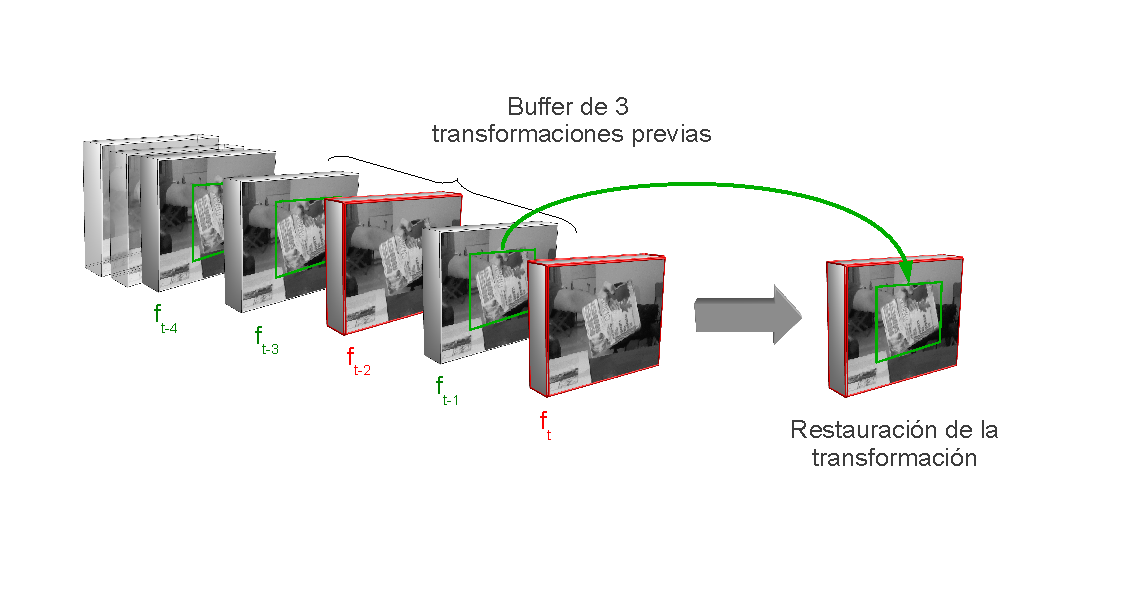
\includegraphics[scale=0.8]{../figs/restauracion_transfromacion}
    \caption[Esquema de restauración de la última transformación válida]{Esquema de restauración de la última transformación válida.}
   \label{fig:restauracion_transformacion} 
\end{figure}

Para el caso donde no se detecta la transformación en ninguno de los últimos tres frames procesados, no se altera el flujo de video y se reinicia el procedimiento capturando una nueva imagen del flujo de video y comenzando así un nuevo ciclo en el método.
%%%%%%%%%%%%%%%%%%%%%%%%%%%%%%%%%%%%%%%%%%%%%%%%%%%%%%%%%%%%%%%%%%%
\section{Realidad aumentada en el flujo de video}
Esta etapa comprende la presentación del resultado final al proceso completo descripto en este capítulo. Como se observa en el diagrama de la Fig. \ref{fig:diagrama_metodo}, el último paso antes de recomenzar el proceso es ``enriquecer la realidad'', que se traduce en actualizar el frame de video sobreponiendo el objeto virtual. El proceso que es llevado a cabo aquí, dependerá de la detección de la imagen patrón en el flujo de video y de la acción que se quiera ejecutar en base a ello.

Para el caso donde no se detecta la imagen patrón en el flujo de video, simplemente se debe dibujar el fotograma del flujo de video para actualizar la escena. Por el contrario, si la imagen fue detectada, se aplica la misma acción establecida anteriormente, pero además se debe superponer el objeto virtual. 
La realidad puede ser modificada utilizando un sinfín de opciones, como ser texto, audio, fotografías, etc., o incluso una combinación de las mismas. Para nuestra aplicación, se propone la modificación del objeto patrón presente en la imagen mediante la reimpresión de otro en su lugar.
% En nuestro caso, se plantea mediante un simple prototipo en el que se dibuja una imagen (``Objeto de realidad aumentada'') sobre la posición detectada. Sin embargo, aquí se puede abrir un sinfín de posibilidades en el que se podrían pensar diferentes clases de recursos como texto, audio, etc. que serán dejados como tema de trabajo futuro para su implementación.

Para superponer el ``objeto de realidad aumentada`` en la posición y perspectiva correcta, se utiliza una Transformación Perspectiva.
%cvWarpAffine estaba mal usado, al transformar un cuadrilatero se desforman las diagonales usando este
\subsection{Transformación Perspectiva}
La transformación perspectiva es un tipo de transformación geométrica, que nos permite realizar un dimensionamiento no uniforme y rotación al objeto de RA que vamos a incluir en la escena.
% basada en matrices de $3x3$ llamadas transformaciones perspectivas u homografías. A pesar que la misma es especificada mediante una simple matriz, la proyección no es un transformación lineal ya que la misma requiere la división por la dimensión final (usualmente Z). %que brindan más flexibilidad el subconjunto de las afines.

La transformación perspectiva está estrechamente relacionada con la proyección perspectiva. Recordemos que esta última, mapea puntos del sistema físico de coordenadas tridimensionales globales en puntos del plano de la imagen en dos dimensiones, a través de un conjunto de líneas de proyección que se intersectan en un punto en común llamado centro de proyección.
La transformación perspectiva es un tipo específico de homografía (homografía plana), que relaciona dos imágenes diferentes, las cuales son proyecciones alternativas del mismo objeto tridimensional sobre dos planos proyectivos diferentes.% (y esto para no degenerar las configuraciones tales como el plano que intersecta físicamente el objeto 3D, típicamente para dos diferentes centros de proyección)

El objetivo aquí es transformar la imagen ``objeto de realidad aumentada'' para luego sobreimprimir en la escena y lograr enriquecer la realidad. La homografía $H$ calculada anteriormente, mapea puntos de una primer imagen a puntos en una segunda imagen. Lo que se necesita para transferir los puntos de la primer imagen a la segunda es la homografía inversa. Sabemos que a partir de la detección del objeto en el flujo de video se obtiene una estimación de $H$, luego para superponer la imagen virtual en la perspectiva correcta en el flujo de video  se utiliza la inversa $(H^{-1})$. Un esquema del proceso puede ser observado en la Fig. \ref{fig:transf_pespectiva}. Como es necesario transformar los píxeles de una imagen en una posición a otra, se debe tener en cuenta una interpolación para dibujar todos los píxeles en la nueva posición.
\begin{figure}[tbhp]
   \centering
        \includegraphics[scale=0.75]{../figs/transfperspectiva}
    \caption[Esquema de transformación perspectiva]{Esquema de transformación perspectiva utilizando la homografía $H$.}
   \label{fig:transf_pespectiva}
\end{figure}
%%
% La proyección perspectiva proyecta puntos de un plano de imagen a lo largo de lineas que se intersectan en un punto común llamado centro de proyección.
Para realizar la transformación perspectiva se utilizó \textit{cvWarpPerspective} \footnote{\url{http://opencv.willowgarage.com/documentation/cpp/imgproc_geometric_image_transformations.html\#cv-warpperspective}} (librería OpenCV) que permite transformar los puntos dada la matriz de homografía, realizando la interpolación mencionada.